% 1998 上海文科第19题：直四棱柱、底面菱形与对角线/辅助线关系；示意图不按比例。
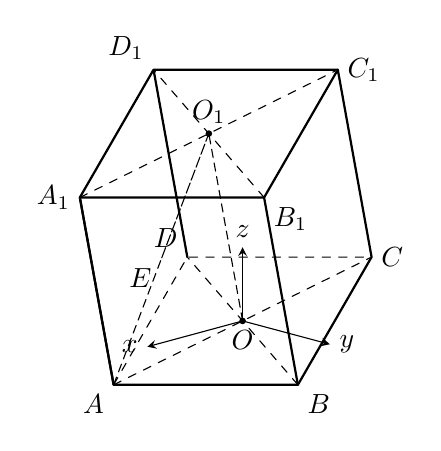
\begin{tikzpicture}[x=0.78cm,y=0.78cm,>=stealth,line cap=round,line join=round]
  \coordinate (A)  at (0,0);
  \coordinate (B)  at (3,0);
  \coordinate (C)  at (4.2,2.08);
  \coordinate (D)  at (1.2,2.08);
  \coordinate (A1) at (-0.55,3.05);
  \coordinate (B1) at (2.45,3.05);
  \coordinate (C1) at (3.65,5.13);
  \coordinate (D1) at (0.65,5.13);
  \coordinate (O)  at (2.1,1.04);
  \coordinate (O1) at (1.55,4.09);
  \coordinate (E)  at (0.775,2.045);
  % 棱柱棱；遮挡部分使用虚线。
  \draw[thick] (A)--(B)--(C)--(C1)--(B1)--(A1)--cycle;
  \draw[thick] (A1)--(D1)--(C1) (D1)--(D);
  \draw[thick] (A)--(A1) (B)--(B1);
  \draw[dashed] (A)--(D)--(C) (D)--(D1);
  % 上下底面对角线及辅助连线。
  \draw[dashed] (A)--(C) (B)--(D) (A1)--(C1) (B1)--(D1);
  \draw[densely dashed] (A)--(O1) (O1)--(E) (O)--(O1);
  \fill (O) circle (1.2pt);
  \fill (O1) circle (1.2pt);
  \node[below left] at (A) {$A$};
  \node[below right] at (B) {$B$};
  \node[right] at (C) {$C$};
  \node[above left] at (D) {$D$};
  \node[left] at (A1) {$A_1$};
  \node[below right] at (B1) {$B_1$};
  \node[right] at (C1) {$C_1$};
  \node[above left] at (D1) {$D_1$};
  \node[below] at (O) {$O$};
  \node[above] at (O1) {$O_1$};
  \node[below left] at (E) {$E$};
  % 坐标轴方向与题面指定一致，仅表示方向。
  \draw[->] (O) -- ++(-1.55,-0.42) node[left] {$x$};
  \draw[->] (O) -- ++(1.42,-0.38) node[right] {$y$};
  \draw[->] (O) -- ++(0,1.2) node[above] {$z$};
\end{tikzpicture}
